\chapter{Beschränkte Systeme und Hamiltonsche Bewegung}

\lectureoverview{Zwei beschränkte Systeme zeigen, weshalb die Lagrangesche Mechanik so wirksam ist: Sobald geeignete Koordinaten gewählt sind, ergeben sich die Bewegungsgleichungen und ihre Erhaltungssätze ohne eine explizite Berechnung der Zwangskräfte. Dieselben Beispiele führen anschließend zur Hamiltonschen Mechanik, in der Koordinaten und Impulse den Phasenraum bilden, der harmonische Oszillator zu einer starren Rotation wird und Hamiltons zwei Gleichungen erster Ordnung jeweils eine Euler--Lagrange-Gleichung zweiter Ordnung ersetzen.}

\section{Was es bedeutet, ein mechanisches Problem zu lösen}

Der unmittelbare Zweck der Lagrange-Methode ist praktischer Natur. Ein auf einem Boden gleitender Keil und ein Doppelpendel lassen sich beide mit den Newtonschen Gesetzen behandeln, doch die unbekannten Kontaktkräfte und Spannungen machen die Rechnung schnell mühsam. Kennt man die Regeln der Lagrangeschen Mechanik, werden dieselben Probleme zu einer Folge überschaubarer Schritte:
\begin{enumerate}
  \item unabhängige Koordinaten wählen, die eine momentane Konfiguration beschreiben;
  \item kinetische und potenzielle Energie in diesen Koordinaten ausdrücken;
  \item \(L=T-V\) aufstellen und die Euler--Lagrange-Gleichungen anwenden.
\end{enumerate}

Für den gegenwärtigen Zweck gilt ein Problem bereits als \emph{gelöst}, wenn seine Bewegungsgleichungen korrekt aufgestellt sind. Vielleicht möchte man noch eine geschlossene Lösung für die Bahnkurve finden, doch das ist eine separate Frage. Nichtlineare Differentialgleichungen lassen sich numerisch integrieren, sobald das mechanische Problem vollständig aufgestellt ist. Die Schwierigkeit liegt oft nicht in der Integration, sondern darin, Variablen zu finden, die die Zwangsbedingungen einbeziehen, ohne redundante unbekannte Kräfte einzuführen.

\section{Ein Teilchen gleitet auf einem beweglichen Keil}

Betrachten wir einen Keil der Masse \(M\), der ohne Reibung auf einer horizontalen Ebene gleiten kann. Ein Punktteilchen der Masse \(m\) ist darauf beschränkt, auf der schiefen Fläche zu bleiben. Es gibt zwei Freiheitsgrade: Einer gibt die Lage des Keils an, der andere die Lage des Teilchens auf dem Keil.

Seien
\begin{equation}
  \begin{aligned}
    X&=\text{horizontal position of the wedge corner},\\
    x&=\text{horizontal displacement of the particle}\\[-0.2em]
     &\phantom{={}}\text{from that corner}.
  \end{aligned}
  \label{eq:l6-wedge-coordinates}
\end{equation}
Die absolute horizontale Koordinate des Teilchens ist somit \(X+x\). Die Wahl ist nicht eindeutig. Stattdessen könnten wir den Abstand entlang der schiefen Ebene oder die absolute horizontale Koordinate des Teilchens verwenden. Jedes nicht redundante Koordinatenpaar, das dieselben Konfigurationen beschreibt, ist zulässig; manche Paare machen die Struktur jedoch deutlicher als andere.

Bei einem festen Neigungswinkel \(\beta\) ist die vertikale Verschiebung \(y\) keine unabhängige Koordinate:
\begin{equation}
  y=x\tan\beta,
  \qquad
  \dot y=\dot x\tan\beta.
  \label{eq:l6-wedge-constraint}
\end{equation}
Wir betrachten den Spezialfall \(\beta=45^\circ\), sodass \(y=x\) und
\(\dot y=\dot x\). Diese Vereinfachung beseitigt trigonometrische Faktoren, ohne die Aussage des Beispiels zu verändern.

\begin{figure}[htbp]
  \centering
  \includegraphics[width=0.84\textwidth]{lecture_06_figure_06.png}
  \caption{Der bewegliche Keil, das an ihn gebundene Teilchen sowie die horizontalen und vertikalen Geschwindigkeitskomponenten, die im Beispiel mit \(45^\circ\) verwendet werden.}
  \lectureframe{00:10:25}
\end{figure}

Die kinetische Energie des Keils ist
\begin{equation}
  T_{M}=\frac{M}{2}\dot X^2.
  \label{eq:l6-wedge-kinetic}
\end{equation}
Die horizontale Geschwindigkeit des Teilchens beträgt \(\dot X+\dot x\), seine vertikale Geschwindigkeit \(\dot x\). Damit ist seine kinetische Energie
\begin{equation}
  T_m=\frac{m}{2}\left[(\dot X+\dot x)^2+\dot x^2\right].
  \label{eq:l6-particle-kinetic}
\end{equation}
Wählen wir \(x=0\) als Nullniveau der Gravitationsenergie, so gilt \(V=mgx\).
Somit folgt
\begin{equation}
  L=\frac{M}{2}\dot X^2
    +\frac{m}{2}\left[(\dot X+\dot x)^2+\dot x^2\right]
    -mgx.
  \label{eq:l6-wedge-lagrangian}
\end{equation}

\begin{figure}[htbp]
  \centering
  \includegraphics[width=0.86\textwidth]{lecture_06_figure_07.png}
  \caption{Die Keilgeometrie, \(V=mgx\) und die beiden Beiträge zur kinetischen Energie, an der Tafel zusammengestellt.}
  \lectureframe{00:14:15}
\end{figure}

\subsection{Der kanonische Impuls ist durch die Lagrange-Funktion definiert}

Die kanonischen Impulse werden durch die Lagrange-Funktion definiert und nicht anhand der Geschwindigkeit eines einzelnen Teilchens erraten:
\begin{align}
  p_X&=\frac{\partial L}{\partial\dot X}
      =M\dot X+m(\dot X+\dot x),
      \label{eq:l6-wedge-pX}\\
  p_x&=\frac{\partial L}{\partial\dot x}
      =m(\dot X+\dot x)+m\dot x.
      \label{eq:l6-wedge-px}
\end{align}
Der erste Ausdruck ist der gewöhnliche horizontale Gesamtimpuls: Der Keil trägt \(M\dot X\) bei, das Teilchen \(m(\dot X+\dot x)\). Hier tritt er als der zur Koordinate \(X\) konjugierte Impuls auf.

\begin{figure}[htbp]
  \centering
  \includegraphics[width=0.86\textwidth]{lecture_06_figure_08.png}
  \caption{Die zu der Keilkoordinate \(X\) und der Relativkoordinate des Teilchens \(x\) konjugierten kanonischen Impulse.}
  \lectureframe{00:18:05}
\end{figure}

Die Lagrange-Funktion hängt nicht explizit von \(X\) ab. Eine horizontale Verschiebung des gesamten Systems bewirkt die Transformation
\begin{equation}
  \delta X=\epsilon,
  \qquad
  \delta x=0.
  \label{eq:l6-wedge-translation}
\end{equation}
Die allgemeine Regel für infinitesimale Symmetrien
\begin{equation}
  \delta q_i=\epsilon f_i(q),
  \qquad
  Q=\sum_i p_i f_i
  \label{eq:l6-noether-rule}
\end{equation}
liefert daher \(Q=p_X\). Gleichbedeutend damit ist, dass \(X\) zyklisch ist und
\begin{equation}
  \dot p_X=\frac{\partial L}{\partial X}=0.
  \label{eq:l6-wedge-conservation}
\end{equation}

Eine entsprechende Symmetrie unter vertikalen Verschiebungen gibt es nicht. Der Keil darf sich nicht vertikal bewegen, und eine Änderung der Höhe des Teilchens verändert die Gravitationsenergie. Der horizontale Impuls ist erhalten; der vertikale Impuls dieses beschränkten Teilsystems ist es nicht.

Für die Relativkoordinate lautet die Euler--Lagrange-Gleichung
\begin{equation}
  \dot p_x=\frac{\partial L}{\partial x}=-mg.
  \label{eq:l6-wedge-force}
\end{equation}
An dieser Stelle musste an der Tafel ein Vorzeichen korrigiert werden. Verlässlich ist es, von \(L=T-V\) auszugehen: Da \(V=mgx\), ist die Ableitung der Lagrange-Funktion \(-mg\). Dass \(x\) als horizontale Verschiebung eingeführt wurde, hebt die Wirkung der Schwerkraft in ihrer Gleichung nicht auf, denn die Zwangsbedingung verknüpft diese horizontale Verschiebung mit der vertikalen Höhe \(y=x\).

Es ist weder eine Normalkraft noch eine Reaktionskraft aufgetreten. Diese Kräfte nehmen genau die Werte an, die zur Aufrechterhaltung der Zwangsbedingungen erforderlich sind. Bei der Newton-Methode würde man sie einführen und zusammen mit den Beschleunigungen bestimmen; durch die verallgemeinerten Koordinaten werden sie überflüssig.

\section{Das Doppelpendel und die Kunst der Koordinatenwahl}

Nun hängen wir zwei Massen von je einer Einheit an zwei masselose Stäbe der Länge eins. Der erste Stab bildet mit der nach unten gerichteten Vertikalen den Winkel \(\theta\). Für den zweiten Freiheitsgrad haben wir die Wahl: Wir können den zweiten absoluten Winkel \(\phi\) oder den Relativwinkel \(\alpha\) zwischen den Stäben verwenden.

Der Relativwinkel macht die Struktur deutlicher. Schalten wir die Schwerkraft vorübergehend aus. Eine starre Rotation des gesamten Systems ändert seine absolute Orientierung, nicht aber den Winkel zwischen den Stäben:
\begin{equation}
  \theta\longrightarrow\theta+\epsilon,
  \qquad
  \alpha\longrightarrow\alpha.
  \label{eq:l6-double-rotation}
\end{equation}
Bei dieser Wahl wirkt die Rotationssymmetrie nur auf eine Koordinate. Andere Koordinatensysteme sind deshalb nicht falsch. Mit dieser Wahl sind die Symmetrie und damit auch die Erhaltungsgröße leichter zu erkennen.

\begin{figure}[htbp]
  \centering
  \includegraphics[width=0.76\textwidth]{lecture_06_figure_09.png}
  \caption{Das Doppelpendel mit \(\theta\) als erstem Absolutwinkel und \(\alpha\) als Winkel des zweiten Stabs relativ zum ersten.}
  \lectureframe{00:29:20}
\end{figure}

Um die kinetische Energie zu bestimmen, verwenden wir vorübergehend kartesische Koordinaten als Hilfsgrößen für die Rechnung. Bei einer nach unten positiven vertikalen Koordinate befindet sich die erste Pendelmasse bei
\begin{equation}
  x_1=\sin\theta,
  \qquad
  y_1=\cos\theta,
  \label{eq:l6-bob-one-position}
\end{equation}
und damit gilt
\begin{equation}
  \dot x_1=\dot\theta\cos\theta,
  \qquad
  \dot y_1=-\dot\theta\sin\theta,
  \qquad
  \dot x_1^2+\dot y_1^2=\dot\theta^2.
  \label{eq:l6-bob-one-velocity}
\end{equation}
Die zweite Pendelmasse befindet sich bei
\begin{align}
  x_2&=\sin\theta+\sin(\theta+\alpha),\\
  y_2&=\cos\theta+\cos(\theta+\alpha),
  \label{eq:l6-bob-two-position}
\end{align}
und beispielsweise gilt
\begin{equation}
  \dot x_2=\dot\theta\cos\theta
  +(\dot\theta+\dot\alpha)\cos(\theta+\alpha),
  \label{eq:l6-bob-two-xvelocity}
\end{equation}
mit einem entsprechenden Ausdruck für \(\dot y_2\).

\begin{figure}[htbp]
  \centering
  \includegraphics[width=0.88\textwidth]{lecture_06_figure_10.png}
  \caption{Hilfsweise eingeführte kartesische Koordinaten für die beiden Pendelmassen. Sie dienen zur Berechnung der Geschwindigkeiten und werden nicht als zusätzliche Freiheitsgrade eingeführt.}
  \lectureframe{00:35:25}
\end{figure}

Die Summe der beiden kinetischen Energien ergibt den konsistenten Ausdruck unten. Der gemischte Term folgt aus
\begin{equation*}
  \cos A\cos B+\sin A\sin B=\cos(A-B).
\end{equation*}
\begin{equation}
  T=\dot\theta^2
    +\frac12(\dot\theta+\dot\alpha)^2
    +\dot\theta(\dot\theta+\dot\alpha)\cos\alpha.
  \label{eq:l6-double-kinetic}
\end{equation}

\begin{classroomqa}
  \audiencequestion{Enthält dieser Ausdruck bereits die kinetische Energie beider Pendelmassen, oder ist ein Faktor ein halb verloren gegangen?
  \lecturetimestamp{00:38:06--00:38:27}}
  \lecturerresponse{Er enthält beide Beiträge. Er ergibt sich aus
  \(\tfrac12(\dot x_1^2+\dot y_1^2+\dot x_2^2+\dot y_2^2)\).
  Zwei gleiche Beiträge ergeben zusammen den ersten Term
  \(\dot\theta^2\); ein Faktor fehlt nicht.}
\end{classroomqa}

Ohne Schwerkraft hängt \(L=T\) nicht explizit von \(\theta\) ab. Daher gilt
\begin{equation}
  \dot p_\theta=\frac{\partial L}{\partial\theta}=0,
  \label{eq:l6-double-angular-conservation}
\end{equation}
und \(p_\theta\) ist der gesamte Drehimpuls. Beachten wir die genaue Bedeutung der Aussage, dass \(\theta\) nicht auftritt: \(\dot\theta\) tritt durchaus auf, die nicht abgeleitete Koordinate jedoch nicht.

Mit der Wiedereinschaltung der Schwerkraft wird die globale Rotationssymmetrie gebrochen. Bei der oben verwendeten Konvention mit nach unten positiver Vertikalrichtung ergibt eine zweckmäßige Wahl des Nullniveaus
\begin{equation}
  V=-g(y_1+y_2)
   =-g\left[2\cos\theta+\cos(\theta+\alpha)\right].
  \label{eq:l6-double-potential}
\end{equation}
Eine additive Konstante änderte daran nichts. Entscheidend ist, dass \(\theta\) nun explizit auftritt, sodass der zugehörige konjugierte Impuls nicht mehr erhalten ist. Die Energie bleibt erhalten, weil die Lagrange-Funktion nicht explizit von der Zeit abhängt.

\begin{classroomqa}
  \audiencequestion{Sollte an der Tafel stehen:
  \(\dot\theta-\dot\alpha\) oder
  \(\dot\theta+\dot\alpha\)?
  \lecturetimestamp{00:43:00--00:43:54}}
  \lecturerresponse{Bei der hier verwendeten Orientierung ist das Pluszeichen erforderlich. Es entspricht der Konvention in Gl.~\eqref{eq:l6-bob-two-position} und wird in der kinetischen Energie in Gl.~\eqref{eq:l6-double-kinetic} beibehalten. Eine Umkehr der Definition des positiven \(\alpha\) ändert die entsprechenden Vorzeichen; dann müssen jedoch alle Vorkommen konsistent angepasst werden. An der Tafel wurden die beiden Konventionen vermischt.}
\end{classroomqa}

\begin{figure}[htbp]
  \centering
  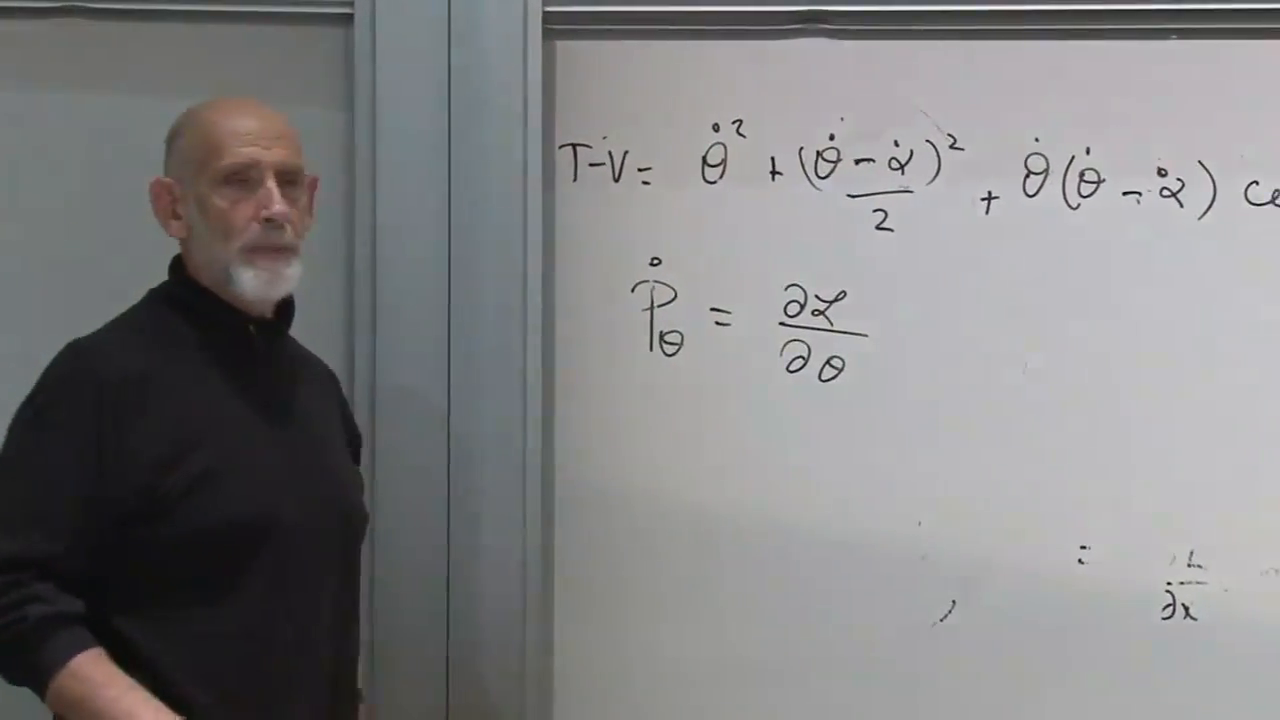
\includegraphics[width=0.84\textwidth]{lecture_06_figure_02.png}
  \caption{Die Pendelrechnung ohne Schwerkraft und \(\dot p_\theta=\partial L/\partial\theta\). Die obere Zeile an der Tafel behält die im Fragebeitrag erörterte, vor Ort vorzeicheninkonsistente Notation bei; die vereinheitlichte Formel steht in Gl.~\eqref{eq:l6-double-kinetic}.}
  \lectureframe{00:45:50}
\end{figure}

Sobald \(T\) und \(V\) bekannt sind, ergeben sich die übrigen Gleichungen durch Ableitung. Auch die Stabspannungen und die Kräfte, die die festen Längen gewährleisten, sind durch die Koordinatenwahl entfallen.

\subsection{Was Erhaltung aussagt und was nicht}

\begin{classroomqa}
  \audiencequestion{Kann man den Gleichungen unmittelbar entnehmen, ob das Doppelpendel chaotisch ist?
  \lecturetimestamp{00:44:57--00:45:25}}
  \lecturerresponse{Meistens lässt sich das nicht durch einfache Betrachtung erkennen. Wenn sich Parameter oder Energien ändern, kann ein System von regelmäßigem zu chaotischem Verhalten übergehen. Um dieses Gebiet zu behandeln, braucht man mehr Struktur als den bloßen Anblick der Gleichungen; es wird später wieder aufgegriffen.}
\end{classroomqa}

\begin{classroomqa}
  \audiencequestion{Ist in einem konservativen System jedes \(\dot p_i\) gleich null?
  \lecturetimestamp{00:45:25--00:46:24}}
  \lecturerresponse{Nein. Die allgemeine Gleichung lautet
  \(\dot p_i=\partial L/\partial q_i\). Sie verschwindet nur, wenn \(q_i\) zyklisch ist. Eine zyklische Koordinate ist der besonders einfache Fall, in dem eine Symmetrie so dargestellt wird, dass sie eine Koordinate verschiebt und die übrigen unverändert lässt.}
\end{classroomqa}

Wenn es allein um die numerische zeitliche Entwicklung geht, funktioniert auch ein unpraktisches Koordinatensystem; es führt lediglich zu längeren Gleichungen. Der Gewinn einer geschickten Wahl ist konzeptioneller Art: Der erhaltene Impuls ist bereits sichtbar, bevor die Gleichungen gelöst werden.

\begin{classroomqa}
  \audiencequestion{Bewegt sich ein Doppelpendel ohne Schwerkraft so einfach wie ein einzelnes freies Pendel?
  \lecturetimestamp{00:47:02--00:47:35}}
  \lecturerresponse{Ein einzelner freier Rotor dreht sich gleichförmig, weil sein einziger Drehimpuls seine Bewegung festlegt. Ein Doppelpendel kann eine sehr komplizierte Relativbewegung ausführen und dabei dennoch den Gesamtdrehimpuls erhalten. Sind anfangs beide Winkelgeschwindigkeiten null, bleibt es in Ruhe; andernfalls wechselwirken die beiden Teile.}
\end{classroomqa}

\begin{classroomqa}
  \audiencequestion{Sind \(\dot\theta\) und \(\dot\alpha\) einzeln konstant, wenn die Schwerkraft fehlt?
  \lecturetimestamp{00:47:36--00:52:42}}
  \lecturerresponse{Nein. Erhaltung bedeutet \(\dot p_\theta=0\), nicht \(\ddot\theta=0\) oder \(\ddot\alpha=0\). Der Ausdruck für \(p_\theta=\partial L/\partial\dot\theta\) enthält beide Winkelgeschwindigkeiten und hängt von \(\alpha\) ab. Die Stäbe übertragen Drehmomente, sodass die beiden Pendelmassen Drehimpuls und Energie austauschen können. Das ist vergleichbar mit zwei durch eine Feder verbundenen Massen: Gesamtimpuls und Schwerpunktsgeschwindigkeit bleiben konstant, während die einzelnen Geschwindigkeiten oszillieren. Das rotatorische Analogon ist eine bestimmte kollektive Kombination, nicht einer der beiden Winkel für sich.}
\end{classroomqa}

\begin{classroomqa}
  \audiencequestion{Werden die Kräfte, durch die Drehimpuls ausgetauscht wird, über die Stäbe übertragen?
  \lecturetimestamp{00:52:43--00:53:34}}
  \lecturerresponse{Ja. Eine entlang eines Stabs übertragene Kraft muss nicht durch den Drehpunkt der anderen Bewegungslinie wirken und kann deshalb ein Drehmoment ausüben. Ein Drehmoment ist schlicht die Drehwirkung einer Kraft; hier führt es zu von null verschiedenen Winkelbeschleunigungen der einzelnen Pendel.}
\end{classroomqa}

\section{Der Hamiltonian als dritte Formulierung}

Der Hamiltonian ist die Energie, doch das ist nur seine erste Bedeutung. Er bildet auch die Grundlage einer dritten Formulierung der Mechanik. Die Newtonschen Gleichungen verwenden Kräfte und Beschleunigungen. Das Prinzip der stationären Wirkung führt zu den Euler--Lagrange-Gleichungen. Für reguläre Systeme ist die Hamiltonsche Mechanik dazu äquivalent, doch ihre Variablen und ihre Geometrie sehen anders aus.

Statt \(q_i\) und \(\dot q_i\) verwenden wir \(q_i\) und die zugehörigen konjugierten Impulse \(p_i\). Zur Beschreibung des Zustands eines Systems mit \(n\) Freiheitsgraden sind in beiden Darstellungen \(2n\) Zahlen erforderlich: entweder Orte und Geschwindigkeiten oder Orte und Impulse. Die Verbindung zwischen ihnen lautet
\begin{equation}
  p_i=\frac{\partial L}{\partial\dot q_i}.
  \label{eq:l6-legendre-map}
\end{equation}
Wenn sich diese Beziehungen nach den Geschwindigkeiten \(\dot q_i(q,p)\) auflösen lassen, definieren wir
\begin{equation}
  H(q,p)=\sum_i p_i\dot q_i-L(q,\dot q).
  \label{eq:l6-hamiltonian-definition}
\end{equation}
Die Geschwindigkeiten auf der rechten Seite werden dann durch \(q\) und \(p\) ersetzt. Diese Umkehrbarkeit ist die Voraussetzung einer regulären Legendre-Transformation. Bei singulären Lagrange-Funktionen ist eine allgemeinere Theorie der Zwangsbedingungen erforderlich; sie wird von dieser elementaren Konstruktion nicht erfasst.

\subsection{Umkehrbarkeit vor der Differentialrechnung}

Betrachten wir eine endliche Menge abstrakter Zustände, die durch Pfeile verbunden sind. Auch eine deterministische Regel kann unumkehrbar sein, wenn zwei frühere Zustände in einen späteren übergehen. Die Zukunft ist eindeutig, die Vergangenheit jedoch nicht. Kehrt man alle Pfeile um, erhält man den entgegengesetzten Fehler: Ein Zustand verzweigt sich in mehrere mögliche Zukünfte. Im ersten Bild laufen die Pfeile zusammen, im zweiten auseinander.

\begin{figure}[htbp]
  \centering
  \includegraphics[width=0.86\textwidth]{lecture_06_figure_11.png}
  \caption{Abbildungen abstrakter Zustände, die umkehrbare Zyklen mit unzulässigem Zusammenlaufen und Auseinanderlaufen vergleichen.}
  \lectureframe{00:56:20}
\end{figure}

Der Hamiltonsche Fluss liefert eine kontinuierliche Entsprechung dieser Aussage. Eine Wolke von Phasenraumpunkten kann sich bewegen und verformen, aber es kann weder eine Senke entstehen, die Unterschiede zwischen Zuständen auslöscht, noch eine Quelle, die aus einem Zustand mehrere Zukünfte hervorbringt. Der Beweis folgt später; vorerst veranschaulichen die Diagramme die Geometrie.

\begin{classroomqa}
  \audiencequestion{Ist das Diagramm der abstrakten Zustände als ein Objekt zu verstehen, das sich in einem Gravitationsfeld bewegt?
  \lecturetimestamp{00:58:02--00:58:35}}
  \lecturerresponse{Nein. Die Punkte stellen lediglich abstrakte Zustände dar, und die Pfeile geben eine Regel für Zustandsänderungen an. Der Zeichnung wurde keine räumliche oder gravitative Bedeutung zugewiesen.}
\end{classroomqa}

\begin{classroomqa}
  \audiencequestion{Wodurch unterscheidet sich eine unzulässige zusammenlaufende Zustandsabbildung von einem Schwarzen Loch?
  \lecturetimestamp{00:58:40--00:59:28}}
  \lecturerresponse{Nur mit Mühe und unter Berücksichtigung feiner Einzelheiten. Die Frage ist berechtigt, doch eine korrekte Antwort erfordert eine sorgfältige Beschreibung des vollständigen Zustands und seiner quantengravitativen Entwicklung. Das elementare Diagramm reicht für eine Entscheidung nicht aus.}
\end{classroomqa}

\section{Ein an den Phasenraum angepasster Oszillator}

Bevor wir die allgemeinen Gleichungen herleiten, betrachten wir einen harmonischen Oszillator in bewusst angepassten Variablen:
\begin{equation}
  L=\frac{1}{2\omega}\dot q^2-\frac{\omega}{2}q^2.
  \label{eq:l6-rescaled-lagrangian}
\end{equation}
Sein konjugierter Impuls ist
\begin{equation}
  p=\frac{\partial L}{\partial\dot q}=\frac{\dot q}{\omega},
  \qquad
  \dot q=\omega p.
  \label{eq:l6-rescaled-momentum}
\end{equation}
Einsetzen in Gl.~\eqref{eq:l6-hamiltonian-definition} ergibt
\begin{align}
  H&=p\dot q-L\\
   &=\omega p^2-\frac{\omega p^2}{2}+\frac{\omega q^2}{2}
    =\frac{\omega}{2}(p^2+q^2).
  \label{eq:l6-oscillator-hamiltonian}
\end{align}

\begin{figure}[htbp]
  \centering
  \includegraphics[width=0.86\textwidth]{lecture_06_figure_12.png}
  \caption{Die Legendre-Transformation des angepassten Oszillators und der symmetrische Hamiltonian \(H=\tfrac{\omega}{2}(p^2+q^2)\).}
  \lectureframe{01:08:20}
\end{figure}

Der Raum der \(q\) und \(p\) ist der Phasenraum. Bei einem Freiheitsgrad ist er eine zweidimensionale Ebene; bei zwei Freiheitsgraden ein vierdimensionaler Phasenraum. Bei fester Oszillatorenergie gilt
\begin{equation}
  p^2+q^2=\frac{2H}{\omega},
  \label{eq:l6-energy-circle}
\end{equation}
sodass die Bahn auf einem Kreis bleibt. Die Energieerhaltung beschränkt die Bewegung auf eine solche Kurve.

\begin{figure}[htbp]
  \centering
  \includegraphics[width=0.82\textwidth]{lecture_06_figure_13.png}
  \caption{Konzentrische Kreise konstanter Energie in der Oszillator-Phasenebene, mit \(q\) auf der Horizontalen und \(p\) auf der Vertikalen.}
  \lectureframe{01:13:20}
\end{figure}

\section{Herleitung der Hamilton-Gleichungen}

Die Herleitung beruht auf dem Differential einer Funktion mehrerer Variablen. Für \(F(q,p)\) gilt:
\begin{equation}
  \delta F=\sum_i\left(
  \frac{\partial F}{\partial q_i}\delta q_i
  +\frac{\partial F}{\partial p_i}\delta p_i\right).
  \label{eq:l6-total-differential}
\end{equation}
Die Koeffizienten lassen sich in beide Richtungen ablesen: Der Koeffizient von \(\delta q_i\) ist \(\partial F/\partial q_i\), und der Koeffizient von \(\delta p_i\) ist \(\partial F/\partial p_i\).

Variieren wir nun den definierenden Ausdruck für \(H\):
\begin{align}
  \delta H
  &=\sum_i\left(\dot q_i\,\delta p_i
       +p_i\,\delta\dot q_i\right)-\delta L\\
  &=\sum_i\left(\dot q_i\,\delta p_i
       +p_i\,\delta\dot q_i
       -\frac{\partial L}{\partial q_i}\delta q_i
       -\frac{\partial L}{\partial\dot q_i}\delta\dot q_i\right).
  \label{eq:l6-vary-hamiltonian}
\end{align}
Da \(\partial L/\partial\dot q_i=p_i\), heben sich die beiden Terme \(\delta\dot q_i\) auf. Die Euler--Lagrange-Gleichungen liefern \(\partial L/\partial q_i=\dot p_i\); damit bleibt
\begin{equation}
  \delta H=\sum_i\left(\dot q_i\,\delta p_i
                     -\dot p_i\,\delta q_i\right).
  \label{eq:l6-reduced-variation}
\end{equation}

\begin{figure}[htbp]
  \centering
  \includegraphics[width=0.86\textwidth]{lecture_06_figure_14.png}
  \caption{Die Ausmultiplizierung der Produktregel für \(\delta H\), bevor sich die Terme \(p_i\,\delta\dot q_i\) aufheben.}
  \lectureframe{01:18:40}
\end{figure}

Vergleichen wir Gl.~\eqref{eq:l6-reduced-variation} mit dem allgemeinen Differential in Gl.~\eqref{eq:l6-total-differential}, so ergeben die unabhängigen Koeffizienten Hamiltons Gleichungen:
\begin{equation}
  \boxed{
  \dot q_i=\frac{\partial H}{\partial p_i},
  \qquad
  \dot p_i=-\frac{\partial H}{\partial q_i}.}
  \label{eq:l6-hamilton-equations}
\end{equation}

\begin{figure}[htbp]
  \centering
  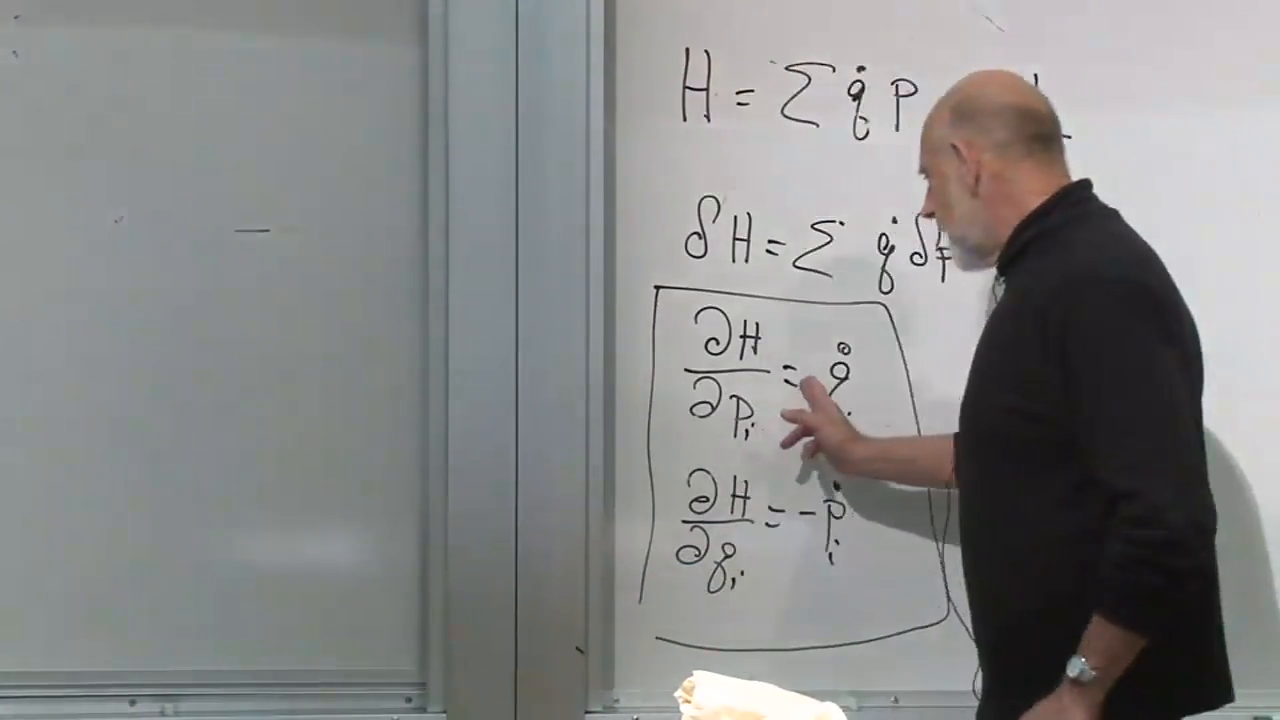
\includegraphics[width=0.78\textwidth]{lecture_06_figure_03.png}
  \caption{Die Definition des Hamiltonians, seine Variation und die eingerahmten kanonischen Gleichungen.}
  \lectureframe{01:22:18}
\end{figure}

Für \(n\) Koordinaten sind dies \(2n\) Gleichungen erster Ordnung. Die Euler--Lagrange-Formulierung liefert dagegen \(n\) Gleichungen zweiter Ordnung. Umfang der Anfangsdaten und physikalischer Gehalt sind identisch.

\section{Die Oszillatorbewegung als starre Rotation}

Wenden wir Gl.~\eqref{eq:l6-hamilton-equations} auf Gl.~\eqref{eq:l6-oscillator-hamiltonian} an, so ergibt sich
\begin{equation}
  \dot q=\omega p,
  \qquad
  \dot p=-\omega q.
  \label{eq:l6-oscillator-first-order}
\end{equation}
Differenzieren wir die erste Gleichung und verwenden die zweite, folgt
\begin{equation}
  \ddot q=\omega\dot p=-\omega^2q.
  \label{eq:l6-oscillator-second-order}
\end{equation}
Die beiden Gleichungen erster Ordnung ergeben also genau die gewöhnliche Oszillatorgleichung zweiter Ordnung, zusammen mit der Definition des Impulses.

Im Phasenraum ist der Geschwindigkeitsvektor am Punkt \((q,p)\) gleich \((\dot q,\dot p)=(\omega p,-\omega q)\) und damit tangential zum Energiekreis. Jeder Radius rotiert mit derselben Winkelgeschwindigkeit \(\omega\). Man kann sich die gesamte Ebene als starres Windrad oder als inkompressible fiktive Flüssigkeit vorstellen. Ihre Punkte kreisen, ohne sich in eine Senke zusammenzudrängen oder von einer Quelle auseinanderzutreiben.

\begin{figure}[htbp]
  \centering
  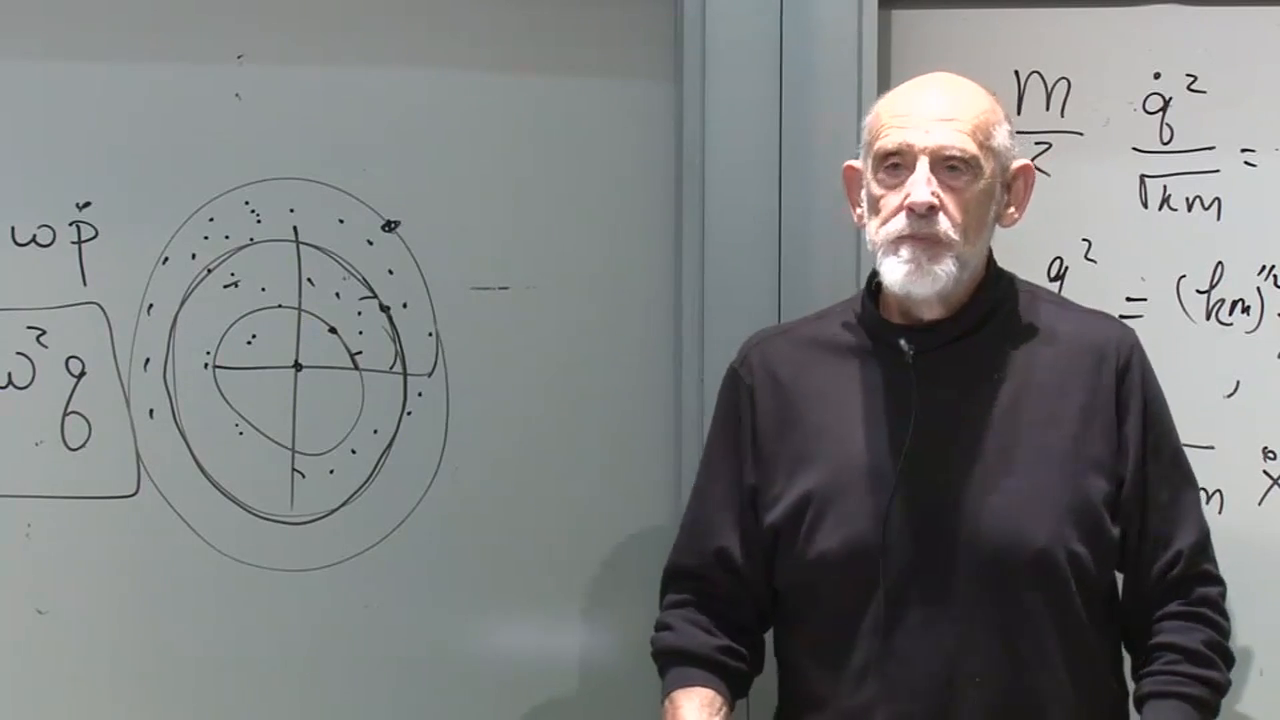
\includegraphics[width=0.86\textwidth]{lecture_06_figure_04.png}
  \caption{Eine Wolke von Anfangspunkten, verteilt auf konzentrische Phasenraumbahnen. Die Hamiltonsche Entwicklung bewegt die Wolke, statt sie in einen ausgezeichneten Zustand kollabieren zu lassen.}
  \lectureframe{01:39:27}
\end{figure}

\begin{figure}[htbp]
  \centering
  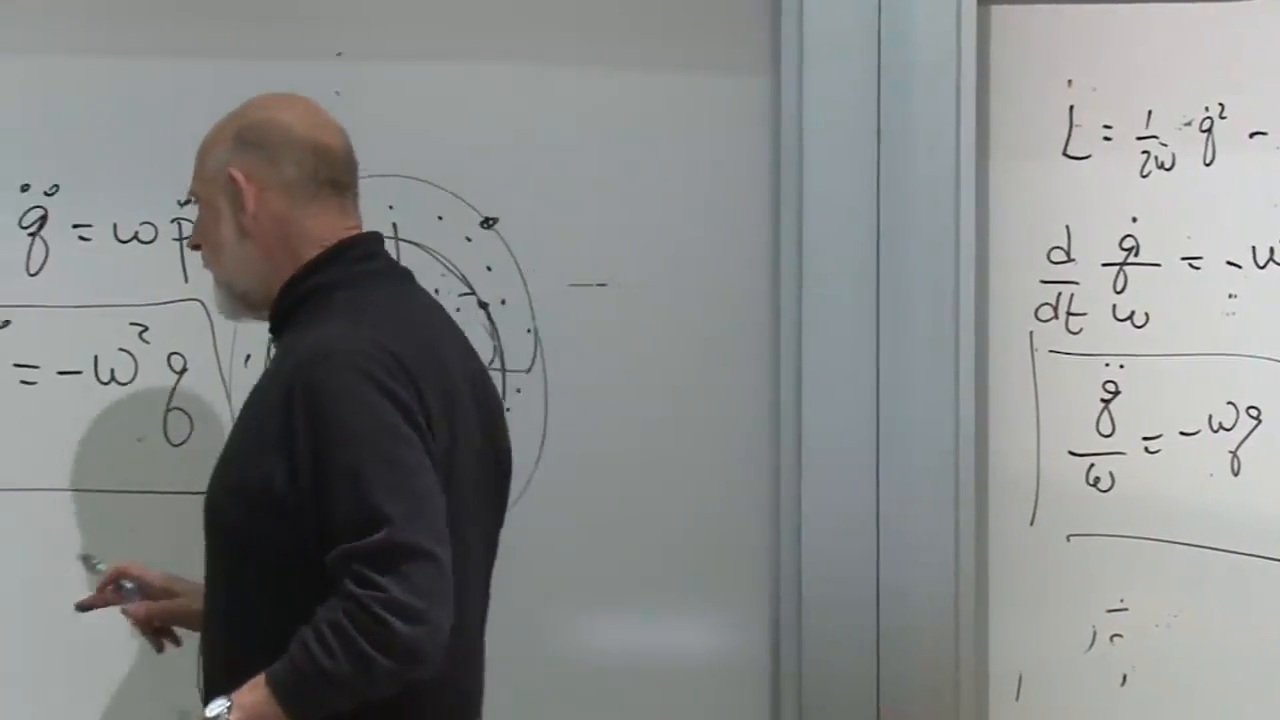
\includegraphics[width=0.90\textwidth]{lecture_06_figure_05.png}
  \caption{Das Phasenportrait des Oszillators neben der äquivalenten Euler--Lagrange-Gleichung
  \(\ddot q/\omega=-\omega q\).}
  \lectureframe{01:42:10}
\end{figure}

Im nächsten Schritt wird die Analogie zur Flüssigkeit zu einem Satz präzisiert: Der Hamiltonsche Fluss weist lokal weder Zusammenlaufen noch Auseinanderlaufen auf. Dieses Ergebnis verknüpft die kontinuierliche Mechanik wieder mit den umkehrbaren Zustandsabbildungen, die zu Beginn des Kurses betrachtet wurden.

\section{Fragen, die die Koordinatenwahl verdeutlichen}

\begin{classroomqa}
  \audiencequestion{Ist die Annahme, dass sich die Geschwindigkeiten durch \(q\) und \(p\) ausdrücken lassen, ein Satz oder eine empirische Eigenschaft physikalischer Systeme?
  \lecturetimestamp{01:29:08--01:29:45}}
  \lecturerresponse{Im Rahmen dieser elementaren Einführung handelt es sich um eine empirische Regelmäßigkeit, für die es eine tiefer gehende Motivation aus der Quantenmechanik gibt. Genauer gesagt muss Gl.~\eqref{eq:l6-legendre-map} eine bezüglich der Geschwindigkeiten nichtsinguläre Jacobi-Matrix haben. Die moderne Mechanik umfasst auch wichtige singuläre Lagrange-Funktionen, insbesondere bei Systemen mit Zwangsbedingungen und Eichsymmetrie; ihre Hamiltonsche Formulierung erfordert jedoch einen zusätzlichen Formalismus für Zwangsbedingungen.}
\end{classroomqa}

Ein Einwand zu den Einheiten erklärt, weshalb der Oszillator in der ungewohnten Form von Gl.~\eqref{eq:l6-rescaled-lagrangian} geschrieben wurde. Beginnen wir stattdessen mit der gewöhnlichen Koordinate \(x\):
\begin{equation}
  L=\frac{m}{2}\dot x^2-\frac{k}{2}x^2,
  \qquad
  \omega=\sqrt{\frac{k}{m}}.
  \label{eq:l6-ordinary-oscillator}
\end{equation}
Wir wählen
\begin{equation}
  q=(km)^{1/4}x.
  \label{eq:l6-oscillator-rescaling}
\end{equation}
Dann gilt \(q^2=\sqrt{km}\,x^2\) und
\(\dot q^2=\sqrt{km}\,\dot x^2\), wodurch Gl.~\eqref{eq:l6-ordinary-oscillator} genau in Gl.~\eqref{eq:l6-rescaled-lagrangian} übergeht. Das neue \(q\) ist eine angepasste verallgemeinerte Koordinate, keine Länge, und sein konjugierter Impuls \(p\) ist nicht der gewöhnliche mechanische Impuls \(p_x=m\dot x\).

\begin{figure}[htbp]
  \centering
  \includegraphics[width=0.86\textwidth]{lecture_06_figure_15.png}
  \caption{Die Skalierung zur Anpassung der Dimensionen: von der gewöhnlichen Oszillatorkoordinate \(x\) zur angepassten Koordinate \(q=(km)^{1/4}x\).}
  \lectureframe{01:36:10}
\end{figure}

\begin{classroomqa}
  \audiencequestion{Wie kann \(\omega p=\dot q\) dimensionskonsistent sein, und weshalb wurden diese Variablen gewählt?
  \lecturetimestamp{01:29:46--01:39:22}}
  \lecturerresponse{Das Symbol \(q\) muss nicht die Dimension einer Länge haben, und sein konjugierter Impuls \(p\) muss nicht die Dimension von \(m\dot x\) haben. Die Skalierung in Gl.~\eqref{eq:l6-oscillator-rescaling} erhält die Dimensionen der Lagrange-Funktion und sorgt dafür, dass \(q\) und \(p\) symmetrisch in \(H\) eingehen. In den ursprünglichen Variablen gilt:
  \[
    H=\frac{p_x^2}{2m}+\frac{kx^2}{2},
  \]
  Die Kurven konstanter Energie sind daher in der \((x,p_x)\)-Ebene Ellipsen. In der angepassten \((q,p)\)-Ebene sind es Kreise. Die Skalierung wurde gewählt, um diese Symmetrie sichtbar zu machen.}
\end{classroomqa}

\begin{classroomqa}
  \audiencequestion{Wie können \(2n\) Hamilton-Gleichungen erster Ordnung äquivalent zu \(n\) Lagrange-Gleichungen zweiter Ordnung sein?
  \lecturetimestamp{01:39:24--01:42:30}}
  \lecturerresponse{Beim Oszillator differenziert man \(\dot q=\omega p\) und setzt \(\dot p=-\omega q\) ein; das Gleichungspaar wird dann zu \(\ddot q=-\omega^2q\). Geht man direkt von der Lagrange-Funktion aus, erhält man
  \[
    \frac{d}{dt}\left(\frac{\dot q}{\omega}\right)
      =-\omega q,
  \]
  also dieselbe Gleichung zweiter Ordnung. Eine der Hamilton-Gleichungen kann als Definition des Impulses über die Geschwindigkeit aufgefasst werden, während die andere dessen zeitliche Entwicklung beschreibt.}
\end{classroomqa}

\section{Warum Phasenraum und potenzielle Energie wichtig sind}

\begin{classroomqa}
  \audiencequestion{Bedeutet die Leistungsfähigkeit des Hamiltonians, dass der Phasenraum eine bessere geometrische Darstellung als der Konfigurationsraum ist?
  \lecturetimestamp{01:42:33--01:44:38}}
  \lecturerresponse{Sie erfüllen unterschiedliche Zwecke. Im Phasenraum lassen sich Zyklen, Flächen konstanter Energie sowie das Ausbleiben von Zusammenlaufen und Auseinanderlaufen besonders deutlich erkennen. Für andere Fragen kann der Konfigurationsraum geeigneter sein. Der tiefere Grund, \(H\) hervorzuheben, liegt darin, dass es in der Quantenmechanik, einem der modernen Gebiete, auf die diese Mechanik hinführt, zu einem zentralen und anschaulicheren Objekt wird.}
\end{classroomqa}

\begin{classroomqa}
  \audiencequestion{Ist die potenzielle Energie als Integral der Kraft aufzufassen?
  \lecturetimestamp{01:44:40--01:45:45}}
  \lecturerresponse{Für konservative Kräfte ist diese Aussage bis auf eine Konstante und bei passender Vorzeichenwahl richtig. Zweckmäßiger ist die umgekehrte Sicht: Man betrachtet das Potenzial als grundlegend und leitet daraus die verallgemeinerte Kraft ab:
  \[
    F_i=-\frac{\partial V}{\partial q_i}.
  \]
  Genau dieser Term tritt in \(\dot p_i=\partial L/\partial q_i\) auf, wenn \(L=T-V\) gilt und die kinetische Energie nicht explizit von \(q_i\) abhängt.}
\end{classroomqa}

\begin{classroomqa}
  \audiencequestion{Welche ungelösten Probleme der modernen Physik soll dieser Weg beleuchten?
  \lecturetimestamp{01:45:46--01:47:47}}
  \lecturerresponse{Der Weg führt zur Quantengravitation und Kosmologie, zur Elementarteilchenphysik einschließlich des Higgs-Sektors und der Neutrinos, zur Relativitätstheorie, Stringtheorie und Quantenfeldtheorie. Die fortbestehende theoretische Aufgabe ist, diese Bestandteile in eine zusammenhängende Struktur einzufügen, insbesondere die Quantenmechanik mit der Gravitation und die Kosmologie mit der Teilchenphysik zu verbinden. Dies beschrieb den Stand der offenen Fragen, wie er sich 2011 darstellte; es war keine Behauptung, ihre Lösung sei bereits bekannt.}
\end{classroomqa}

Die beiden Beispiele mit Zwangsbedingungen und der Oszillator fügen sich nun zu einem Gesamtbild. Verallgemeinerte Koordinaten beseitigen unnötige Kräfte. Symmetrien bestimmen die erhaltenen kanonischen Impulse. Die Legendre-Transformation ersetzt Geschwindigkeiten durch Impulse, und Hamiltons Gleichungen beschreiben die Dynamik als Fluss im Phasenraum. Beim Oszillator ist dieser Fluss eine starre Rotation; bei einem allgemeinen System liefert seine Geometrie die präzise kontinuierliche Bedeutung umkehrbarer Bewegung.